\documentclass[a4paper,10pt]{article}

% Paquetes requeridos
\usepackage[utf8]{inputenc}
\usepackage[T1]{fontenc}
\usepackage[spanish]{babel}
\usepackage{csquotes}
\usepackage{amsmath, amssymb, amsfonts}
\usepackage{graphicx}
\usepackage[style=apa, backend=biber, natbib=true, language=spanish, url=true]{biblatex}
\usepackage{tocloft} % Para personalizar el índice
\usepackage[left=3.5cm,right=2.5cm,top=3.5cm,bottom=3.8cm]{geometry}
\usepackage{setspace} % Espaciado
\usepackage{titlesec} % Para personalizar los títulos
\usepackage{fancyhdr} % Para personalizar encabezados y pies de página
\usepackage{newtxtext}
\usepackage{ragged2e}
\usepackage{caption}
\pagestyle{fancy}
\fancyhf{} % Limpia encabezados y pies de página
\renewcommand{\headrulewidth}{0pt} % Elimina la línea del encabezado
% Configuración para las etiquetas de figura
\captionsetup[figure]{labelformat=empty} % Esto elimina el número de figura y el separador

\addbibresource{referencias.bib}
\DeclareLanguageMapping{spanish}{spanish-apa}
% Configuraciones
\setlength{\parskip}{6pt} % Espacio entre párrafos
\setstretch{1.15} % Espacio entre líneas

\renewcommand{\cftsecleader}{\cftdotfill{\cftdotsep}} % Para puntos en el índice

% Estilos para títulos y subtítulos
\titleformat{\section}
{\normalfont\fontsize{12}{15}\bfseries}{\thesection}{1em}{}
\titleformat{\subsection}
{\normalfont\fontsize{10}{13}\bfseries}{\thesubsection}{1em}{}
\titleformat{\subsubsection}
{\normalfont\fontsize{10.5}{13}\bfseries}{\thesubsubsection}{1em}{}

\usepackage[hypertexnames=false, colorlinks=true, 
linkcolor=blue, 
citecolor=blue, 
urlcolor=blue, 
linkbordercolor={1 1 0}, 
citebordercolor={1 1 0}, 
urlbordercolor={1 1 0}, 
filecolor=blue, 
pdfborderstyle={/S/U/W 1}]{hyperref}

% Inicio del documento
\begin{document}
	\pagestyle{empty}
	% Carátula
	\begin{titlepage}
		\centering
		\vspace*{1.5cm}
		{\fontsize{14}{17}\bfseries Criptografía ligera\par}
		{\small Martin Borgo, Isaías Reniero, Leandro Molina\par}
		{\normalsize Universidad Nacional de Entre Ríos\par}
		{\normalsize Facultad de Ciencias de la Administración\par}
		{\normalsize Licenciatura en Sistemas\par}
		{\small \href{mailto:martinborgo8@gmail.com}{martinborgo8@gmail.com}, \href{mailto:isa.reniero001@hotmail.com}{isa.reniero001@hotmail.com}, \href{mailto:LeandroRodrigoMolina@gmail.com}{LeandroRodrigoMolina@gmail.com}\par}
		{\small \justify\textbf{Abstract.} La criptografía ligera (Lightweight Cryptography), es una rama de la criptografía que se enfoca en desarrollar algoritmos eficientes y de bajo consumo para su implementación en sistemas con recursos limitados, como sistemas embebidos, dispositivos IoT (Internet de las cosas) y microcontroladores. La ausencia de medidas de seguridad adecuadas en tales sistemas genera preocupaciones, especialmente cuando se trata de gestionar información sensible, en este contexto la criptografía ligera ofrece soluciones que permiten proteger eficazmente los datos y las comunicaciones, sin sacrificar la eficiencia de los recursos. En este artículo se recopilan los distintos conceptos, avances y tendencias que se fueron dando a lo largo de los años en este campo de la criptografía.\par}
		
		{\small \justify\textbf{Keywords:} Criptografía Ligera, Block Ciphers, IoT, Seguridad. \par}
	\end{titlepage}
	
	\section{Introducción}
	La criptografía ligera (rama de la criptografía) es uno de los temas de la actualidad que se encuentra en auge. Es usada en dispositivos donde su poder de cómputo es reducido, a este tipo de dispositivos se les conoce como IoT (Internet of Things o Internet de las Cosas), aunque en sus inicios recibía el nombre de red de sensores. Muchos de estos dispositivos utilizan microcontroladores de muy bajo consumo que solo pueden permitirse una pequeña parte de su cómputo a la seguridad\footnote{Es importante tener en cuenta que, aunque la criptografía ligera es útil para dispositivos con recursos limitados, los avances en la tecnología a menudo influyen en lo que se considera "ligero". Ya que lo que se considera ligero en un momento dado podría no serlo en un futuro, a medida que la capacidad de los dispositivos mejore.}. Esto provoca que los algoritmos clásicos de criptografía avanzada no puedan ser usados, debido a la alta latencia y consumo de energía que presentan en estos dispositivos. La criptografía ligera nos brinda una gran variedad de algoritmos “livianos” que han sido diseñados para garantizar confidencialidad, autenticidad e integridad de los datos en los dispositivos IoT. Son algoritmos desarrollados por los ámbitos académicos, agencias estatales o propietarios, los cuales eran empleados en sus inicios, en el área industrial:
	\begin{quote}
		''Un ejemplo común de este uso es el de las redes de sensores. Estas redes tienen como objetivo conectar grandes cantidades de sensores muy simples a un centro principal. Estos sensores funcionan con baterías y/o generarían su propia energía utilizando, por ejemplo, paneles solares. Los algoritmos criptográficos deben usarse en los canales de comunicación entre los sensores y su centro para proporcionar seguridad, autenticidad e integridad de los mensajes. Sin embargo, debido a la muy baja energía disponible y porque la seguridad es un gasto adicional a la funcionalidad real del dispositivo, los algoritmos criptográficos deben ser lo más ‘pequeños’ posible.'' \parencite[1]{biryukov2017state}
	\end{quote}
	\section{Desarrollo de Trabajo}
	\subsection{Estandarización de la Criptografía Ligera: ISO/IEC 18033 y 29192}
	Debido a la gran relevancia que estaban adquiriendo este tipo de algoritmos de encriptación, en 2011 se estandarizan gran parte de estos a través de la creación de la ISO/IEC 18033, que en sus diferentes incisos quedan descritos y especificados cada uno de los métodos de encriptación que estaban siendo utilizados a nivel industrial, académico y gubernamental hasta día de hoy. Aunque el paso más grande se dio en 2012 con la salida de la ISO/IEC 29192-1:2012 donde se introduce por primera vez el término criptografía ligera, brindando definiciones y estableciendo una serie de requerimientos de seguridad, implementación y clasificación. De la mano de la estandarización vienen un conjunto de ventajas, de las cuales \textcite{eterovic15stream} mencionan las siguientes:
	\begin{enumerate}
		\item La libre disponibilidad del algoritmo para su uso. 
		\item Contar con una descripción detallada de las funciones que lo conforman, como así también del diseño en general. 
		\item Poder realizar una verificación del funcionamiento y conformidad mediante un grupo independiente de expertos. 
		\item La existencia de vectores de prueba\footnote{Los vectores de pruebas son un conjunto de datos de entrada predefinidos y conocidos, utilizados para probar y verificar el correcto funcionamiento de un algoritmo.} para corroborar el buen funcionamiento de estos.
	\end{enumerate}
	\subsection{Clasificación y Consideraciones en el Diseño}
	\label{sec:clas_consDiseño}
	\textcite{wehbe2022criptografia} realiza una clasificación de los distintos algoritmos de encriptación, dividiéndolos en 4 grandes grupos:
	\begin{enumerate}
		\item \textbf{Stream ciphers (cifrados de flujo): }Es un cifrado simétrico que opera con una transformación que varía con el tiempo en dígitos individuales de texto plano. Una secuencia de texto plano se cifra usando una secuencia pseudoaleatoria, generada a partir de una clave secreta y un parámetro público. Cada dígito cifrado se obtiene combinando el dígito correspondiente de texto plano con esta secuencia.
		\item \textbf{Block ciphers (cifrados de bloque):} Es un cifrado simétrico que, para una clave específica $k$, define un algoritmo de cifrado que convierte un bloque de texto plano de $n$ bits en un bloque de texto cifrado de $n$ bits, y un algoritmo de descifrado correspondiente.
		\item \textbf{Funciones de hashing criptográficas: }Toman cadenas de entrada de longitud arbitraria y las convierten en cadenas de salida de longitud fija y corta, que es única (en teoría) para cada entrada única.
		\item \textbf{Algoritmos de criptografía asimétrica (Sistemas de clave pública, como RSA y curvas elípticas): }Utiliza claves diferentes para cifrar y descifrar. Una clave puede ser pública, mientras que su contraparte debe mantenerse en secreto.
	\end{enumerate}
	En la actualidad se proponen muchos algoritmos criptográficos donde sus diseños varían mucho, y cuya única similitud es la baja potencia requerida para su ejecución. La implementación o diseño de estos algoritmos están divididos en dos: hardware y software. Independientemente de eso, al momento de su diseño se debe hacer hincapié en el consumo de memoria, el tamaño de la implementación (código o circuitería requerida) y la velocidad del algoritmo. Lo que sí varía de un tipo de implementación a otra son los parámetros utilizados para indicar su eficiencia. Más allá de esos aspectos, no importa la implementación específica que se haga, ya que un algoritmo de criptografía ligera debe, idealmente, conseguir un equilibrio entre seguridad, rendimiento y costo. A continuación, mencionaremos los aspectos principales en los que se deben enfocar cada uno de los diseñadores e implementadores de acuerdo con el tipo de implementación particular por la que se haya decantado
	
	Si se desea realizar una implementación por hardware, para que este sea eficiente se deben tener en consideración los siguientes puntos:
	\begin{itemize}
		\item Debe minimizar el consumo de memoria, en RAM o el área de puerta en dispositivos con recursos limitados.
		\item El tamaño de la implementación debe ser optimizado, es decir, que el diseño debe ser lo más compacto posible para ocupar menos espacio en el chip.
		\item Debe considerar el acceso a la memoria no volátil y cómo se accede a las claves almacenadas en ella.
		\item Las operaciones como las permutaciones de bits, que son baratas en hardware, son las más preferidas.
		\item La estructura de la clave no debe requerir un estado de clave que se actualice en cada ronda, ya que esto sería costoso en términos de área de puerta.
	\end{itemize}
	Si la implementación que se desea realizar es de software, para que este sea eficiente se deberá considerar los siguientes puntos:
	\begin{itemize}
		\item Debe minimizar el consumo de memoria, en RAM utilizada.
		\item Las operaciones como las rotaciones de palabras, que son eficientes en software, pueden ser preferidas.
		\item Debe considerar la forma en que se accede a las claves y cómo se almacenan en la memoria.
		\item Las operaciones que son inherentemente costosas en software, como el manejo de bits a nivel individual, deben evitarse o minimizarse.
		\item Las estructuras de clave que pueden evaluarse "en el momento", es decir, generadas en tiempo real durante la ejecución en lugar de pre-calculadas y almacenadas son preferibles para mantener la eficiencia.
	\end{itemize}
	\subsection{Algoritmos Criptográficos Ligeros: Tendencias y Desafíos}
	\textcite{biryukov2017state} enumeran algunas de las tendencias que se están adoptando en el diseño de nuevos algoritmos criptográficos ligeros, donde se mencionan las operaciones no lineales, operaciones lineales y se discute sobre el esquema de llaves.
	
	Las operaciones no lineales son realmente necesarias en cualquier algoritmo de encriptación, ya que brindan una mayor protección contra ciertos ataques, concretamente los ataques de criptoanálisis\footnote{El criptoanálisis se centra en estudiar y analizar los sistemas criptográficos para poder vulnerar su seguridad, algunas de las técnicas usadas son el reconocimiento de patrones de redundancia de los textos, el averiguar características del algoritmo de cifrado, entre otras.}, los ataques de fuerza bruta\footnote{En los ataques de fuerza bruta se trata de descubrir la clave utilizada para cifrar la información, probando todas las combinaciones posibles, es un mecanismo útil cuando se sabe que las llaves de cifrado son cortas.} y los ataques de canal lateral\footnote{Un ataque de canal lateral se centra en el análisis de la información indirecta que se filtra durante el proceso de cifrado o descifrado, con el objetivo de descubrir información sensible o claves de seguridad. Esta información puede ser la variación en el consumo eléctrico, el tiempo de respuesta del dispositivo, entre otros.}. Dentro de los mecanismos utilizados en la criptografía ligera se encuentran las tablas de consultas (Look-up Table), las cuales son una estructura de datos que, suele ser implementada a través de cajas de sustitución\footnote{Las S-Boxes son funciones booleanas vectoriales no lineales, que toman un número determinado de bits de entrada y los transforman en otro número de bits de salida, que no necesariamente tiene que ser la misma cantidad de bits.} (S-Boxes), estas se utilizan para realizar operaciones no lineales de manera más eficiente, y debido que pueden ser implementadas utilizando S-Boxes, permiten que los algoritmos que utilizan estas tablas puedan ser eficientemente implementados tanto por hardware como por software. Se menciona también a los algoritmos basados en segmentos de bits, que utilizan S-Boxe de manera distinta, permitiéndole realizar operaciones bit a bit como AND y XOR, en palabras de w bits. Dado que esta tarea requiere un número limitado de operaciones lógicas, los algoritmos que utilizan esta técnica se destacan por su eficiencia en la implementación por software y hardware. Por último, se encuentran los algoritmos basados en ARX (adición, rotación y XOR), que, debido a su simplicidad, eficiencia y a la gran dispersión en los datos que se consigue con ellos, junto con el hecho de que la adición a nivel de software es extremadamente eficiente, hace que los algoritmos basados en ARX se encuentran entre los mejores en rendimiento para microcontroladores.
	
	Las operaciones lineales, por otro lado, tienen un rol fundamental, ya que proveen de difusión a los datos. Entre los mecanismos mencionados por los autores se encuentran las matrices de máxima distancia separable (MDS Matrix), las cuales proveen una dispersión adecuada de los datos, al mismo tiempo que minimiza el costo computacional, aumentando la protección contra criptoanálisis lineales y diferenciales. La permutación de bits es otro mecanismo que está siendo altamente utilizado en ciertas plataformas, debido a que, en términos generales, su implementación por hardware se puede realizar a bajo costo, con el inconveniente que por el momento son un poco costosas de realizarse a nivel software, es por esa razón que son mayormente empleados por dispositivos RFID y similares. Por último, nombran a los algoritmos que se basan en rotación y XOR (RX), estos brindan una difusión apropiada, siendo barato de implementar tanto por software como por hardware, acarreando casi todas las ventajas de los algoritmos basados en ARX, pero con un menor costo.
	
	Los autores finalizan hablando de las claves de encriptación, y debido a su elevado consumo en términos de RAM, hace que los diseñadores opten por implementar estos algoritmos utilizando claves de corta extensión, dejándolos expuestos a ataques de llaves relacionadas\footnote{Los ataques de claves relacionadas son un tipo de ataque criptográfico en el cual se intenta comprometer la seguridad en el cifrado aprovechándose de la relación existente entre las diferentes claves utilizadas en el sistema. Estos ataques se basan en el hecho de que ciertos algoritmos criptográficos pueden exhibir vulnerabilidades cuando se utilizan claves relacionadas de alguna manera específica.}y ataques de fuerza bruta. Si bien en la actualidad existen una serie de algoritmos que se jactan de ser inmunes a este tipo de ataques, esto lo consiguen añadiendo más rondas al momento de encriptar los datos o a través de esquemas de llaves más complejos, en ambos casos este tipo de alternativas no es muy preferida a la hora de crear este tipo de algoritmos. Por esta razón nacen los distintos esquemas de llaves, cuya principal función es diversificar y distribuir la clave principal en subclaves que se utilizan en diferentes rondas o etapas del cifrado para mejorar la seguridad y la resistencia a diversos tipos de ataques. Aunque al momento de la implementación se puede emplear este mecanismo de diversas formas:
	\begin{itemize}
		\item Utilizar una variante más sencilla del esquema de llaves para solventar los problema de seguridad referidos a ataques relacionales.
		\item Proporcionar una mayor seguridad mediante un esquema de llaves mucho más complejo.
		\item Generar subclaves a partir de una clave maestra, tomando diferentes grupos de bits de la clave maestra.
		\item Utilizar la función de rotación para actualizar el estado de la clave original.
	\end{itemize}
	La tabla \ref{algoritmosCriptografiaLigera} ofrece en forma de ejemplo, algunos de los algoritmos más populares que utilizan cada una de las técnicas antes mencionadas. Hay que tener en cuenta que algunos algoritmos pueden estar en más de una categoría debido a que existen diferentes implementaciones de este.
	\begin{itemize}
		\item Tabla de consultas (Look-up Table): TC
		\item Segmentos de bits (Bit-slice): ASB
		\item ARX (adición, rotación y XOR): ARX
		\item Matrices de máxima distancia separable (MDS Matrices): MDS
		\item Permutación de bits (Bit Permutations): PB
		\item Rotación y XOR (RX): RX
		\item Utilizan una variante sencilla del esquema de llaves: AV
		\item Utilizan esquemas de llaves más elaborados: AEE
		\item Generan subclaves a partir de una clave principal: ASP
		\item Cambian el estado de las claves a partir de una función de rotación: AR	
	\end{itemize}
	\begin{figure}[h]
		\centering
		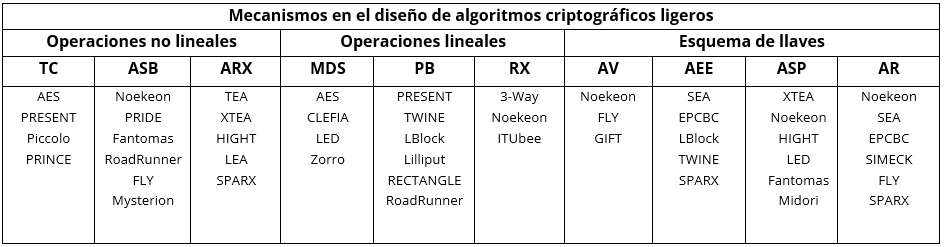
\includegraphics[width=1.0\textwidth]{tablaAlgoritmosCriptografiaLigera.PNG}
		\caption{Tabla 1: Algoritmos que usan mecanismos de diseño}
		\label{algoritmosCriptografiaLigera}
	\end{figure}

	\section{Resultados Obtenidos y Esperados}
	En la sección \ref{sec:clas_consDiseño} se clasificó todas las formas existentes de encriptación. Si bien todos estos esquemas son utilizados para una amplia gama de propósitos, cuando hablamos de algoritmos ligeros, el esquema asimétrico y las funciones hash suelen ser descartadas, ya que las primeras, en términos generales, son muy costoso y las segundas son empleadas para otro tipo de propósitos como la validación de datos o la construcción de primitivos criptográficos. Es por eso que a la hora de diseñar un algoritmo ligero se opta por los esquemas de encriptación simétrica, es decir, modelos basados en Block cipher o Stream cipher, la tabla \ref{Diferencias_Block_Stream_Cipher} muestra las principales diferencias entre estos dos modelos:
	
	En general se utilizan algoritmos basados en Block Cipher cuando el tamaño de los datos es fijo o es conocido de antemano, algunos de sus usos son, por ejemplo, en el protocolo SSL/TLS que utilizan cifrado de bloque para proteger la comunicación entre el cliente y el servidor. Por otro lado, se utiliza un cifrado de flujo cuando los datos a cifrar poseen un tamaño muy variable e imposible de predecir, protocolos Wi-Fi como el WEP o WPA e incluso las comunicaciones satelitales utilizan este tipo de algoritmos. \textcite{thakor2020lightweight}, menciona otras de las áreas donde se emplean este tipo de algoritmos, entre ellas:
	\begin{itemize}
		\item En dispositivos eléctricos que se utilizan en el hogar, como televisores inteligentes, refrigeradores y otros dispositivos similares, que implementan algoritmos como SIMON, SPECK, Piccolo y TWINE. 
		\item En el ámbito de la logística y la gestión de la cadena de suministro mediante la tecnología RFID (Identificación por Radiofrecuencia), que utilizan algoritmos como SIMON, SPECK, Piccolo y PRINCE.
		\item En el uso de sensores en la agricultura inteligente para monitorear y controlar aspectos de la producción agrícola, en los cuales se aplican algoritmos como SIMON, SPECK, PRESENT y TWINE.
		\item En el uso de sensores en el campo de la medicina para la monitorización y el seguimiento de la salud de los pacientes, donde se utilizan algoritmos como SIMON, SPECK, PICCOLO y PRESENT.
		\item En los sistemas industriales en entornos de fabricación, producción y procesamiento, que hacen uso del algoritmo AES.
		\item La incorporación de sistemas de seguridad y comunicación en la industria automotriz que utilizan los algoritmos Keeloq, Midori, PRINCE, PRESENT y SIMON\footnote{Para su mayor conocimiento, en el mismo artículo se enumera una serie de algoritmos ligeros junto con los tipos de ataques a los que han sido sometido cada algoritmo. Los tipos de ataques incluyen ataques de criptoanálisis, ataques de canales laterales, ataques de fuerza bruta, entre otros. Esta información resulta útil para comprender la seguridad de los algoritmos y evaluar su resistencia a diversos tipos de amenazas.}.
	\end{itemize}
	\begin{figure}[h]
		\centering
		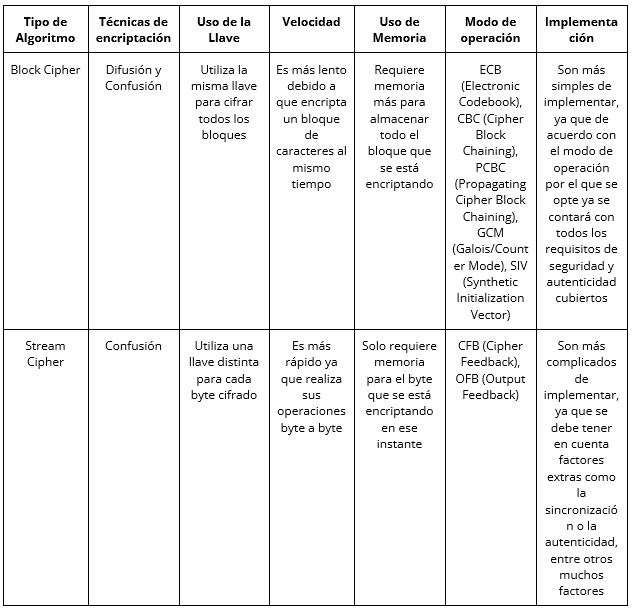
\includegraphics[width=1.0\textwidth]{tablaBlockStreamCipher.PNG}
		\caption{Tabla 2: Diferencias entre Block y Stream cipher}
		\label{Diferencias_Block_Stream_Cipher}
	\end{figure}
	\section{Conclusión}
	
	\section{Referencias}
	\nocite{*}
	\printbibliography[heading=none]
\end{document}
